\documentclass[a4paper,11pt] {article}
\usepackage[spanish]{babel}
\usepackage[utf8]{inputenc}
\usepackage{caratula}
\usepackage{a4wide}
\usepackage{graphicx}
% \usepackage{dot2texi}
% \usepackage{graphs}

\begin{document}

\titulo{Trabajo Pr\'actico Nro. 2}
\fecha{08/05/2009}
\materia{Algoritmos y Estructuras de Datos III}
\grupo{}
\integrante{Dinota, Mat\'ias}{076/07}{matiasgd@gmail.com}
\integrante{Huel, Federico Ariel}{329/07}{federico.huel@gmail.com}
\integrante{Leveroni, Luciano}{360/07}{lucianolev@gmail.com}
\integrante{Mosteiro, Agust\'in}{125/07}{agustinmosteiro@gmail.com}

\maketitle

\bigskip
\section*{Aclaraci\'ones generales}

Antes de comenzar el an\'alisis de cada ejercicio, cabe mencionar lo siguiente:

\begin{itemize}
 \item La implementaci\'on de los 3 algoritmos se realiz\'o en \textbf{lenguaje Java}, haciendo uso de las librer\'ias est\'andar del mismo.
 \item Para el c\'alculo de tiempo de los algoritmos se utiliz\'o la funci\'on \textbf{nanoTime()} de la clase System de Java. Con el fin de aumentar la precisi\'on de las mediciones, se utiliz\'o el comando \textbf{nice} para darle m\'axima prioridad a la tarea.
 \item El c\'odigo fuente de los algoritmos aqui analizados se encuentran en los archivos \textit{Dengue.java} (Ej 1), \textit{...} (Ej 2) y \textit{...} (Ej 3).
 \item El c\'odigo fuente de los programas encargados de hacer uso de los algoritmos y necesarios para compilar las aplicaciones son:
 \begin{itemize}
    \item \underline{Ej 1:} MainDengue.java, Dengue.java e InstanciaDengue.java.
    \item \underline{Ej 2:} ...
    \item \underline{Ej 3:} ...
  \end{itemize}
 \item Para la lectura y escritura de los datos se utilizaron clases provistas por el lenguaje Java. No se har\'a referencia a estos algoritmos ya que no resultan de inter\'es para el trabajo aqui presentado.
 \item Al ejecutar cada programa sin argumentos se muestra una leyenda explicando su modo de uso.
 \item Los gr\'aficos se realizaron con \textbf{GNUPlot}. En los casos considerados pertinentes, se utiliz\'o una escala logar\'itmica con el fin de poder visualizar mejor los resultados.
\end{itemize}

\begin{center}
\section*{Ejercicio 1: Dengue}
\end{center}

\bigskip
\section*{Introducci\'on}

El objetivo del siguiente ejercicio es diseñar un algoritmo que resuelva el problema planteado de manera polinomial. Para esto se utiliz\'o la t\'ecnica de progamaci\'on din\'amica, lo que implic\'o la realizaci\'on de diversos pasos. Primero se corrobor\'o que el problema cumpla con el principio de optimalidad. Una vez comprobado esto (condici\'on necesaria para poder aplicar programaci\'on din\'amica) y utilizando las ideas vistas en dicha demostraci\'on, se procedi\'o a crear una funci\'on recursiva que retorne el resultado deseado. Luego se modific\'o dicha version por un algoritmo iterativo, siendo este un paso intermedio requerido para aplicar la t\'ecnica mencionada. El paso siguiente consisti\'o en modificar el algoritmo de manera de evitar la repetici\'on de c\'alculos innecesarios (aqu\'i queda implicita la idea de programaci\'on din\'amica), mejorando notablemente la complejidad de la funci\'on. Por \'ultimo, como veremos m\'as adelante, se opt\'o por un cambio de t\'ecnica algoritmica pasando de un algoritmo que originalmente era \textit{top-down} a uno \textit{bottom-up}.

\section*{Algoritmo}

En la presente secci\'on presentaremos todos los pasos que se siguieron para lograr la implementaci\'on del algoritmo que resuelve el problema. Como se mencion\'o anteriormente, el problema ser\'a resuelto por medio de la t\'ecnica de programaci\'on din\'amica por lo que presentaremos las demostraciones de todos los pasos que implica construir un algoritmo de esa manera. En primer lugar, se demostrar\'a c\'omo aplica el principio de optimalidad en el problema dado. En segundo lugar, plantearemos una funci\'on recursiva que resuelva el problema y demostraremos su correctitud. Finalmente, mostraremos el algoritmo construido con programaci\'on din\'amica, explicando detalladamente por qu\'e resuelve el problema de manera m\'as eficiente que la soluci\'on recursiva.

\subsection*{Principio de optimalidad}

Demostraremos por qu\'e vale el principio de optimilidad en este problema por el absurdo.

Sean $n$ y $l$ la cantidad de zonas y litros disponibles respectivamente y que las zonas se numeran de $1$ a $n$. Suponemos que la cantidad de mosquitos muertos con $l$ litros hasta la zona $n$ es \'optima y llamaremos $P$ a dicha cantidad. Sea $k$ la cantidad de litros usados en la zona $n$, suponemos que hasta la zona $n-1$ usando $l-k$ litros la cantidad de mosquitos muertos ($Q$) no es \'optima y se intenta llegar a un absurdo.

Si hasta la zona $n-1$ la cantidad de mosquitos muertos no es \'optima (para $l-k$ litros), existe otra forma de distribuir los $l-k$ litros entre las zonas $1$ a $n-1$ que hace que la nueva cantidad, a la que llamaremos $R$, sea \'optima (es decir, $R > Q$). Entonces tenemos que

$R + cantMM(n,k) > Q + cantMM(n,k) = P \Rightarrow R + cantMM(n,k) > P$

Esto es un absurdo ya que supusimos que $P$ era la cantidad \'optima. Este absurdo surge de suponer que la cantidad de mosquitos muertos hasta la zona $n-1$ con $l-k$ litros no era \'optima. Entonces queda demostrado que vale el principio de optimalidad para el problema planteado.

\subsection*{Soluci\'on recursiva y demostraci\'on de correctitud} %TODO!!!!!!!!!!!!!!!!!!!!!

A partir de la idea presentada en la secci\'on anterior se puede plantear la siguiente funci\'on recursiva para resolver el problema.
$\\ f(0, l) = 0 \\$
$ f(i,l) = max \left\{ \begin{array}{ll}
         f(i-1,l) & \mbox{$$}\\
        f(i-1, l-k) + MM[i][k] & \mbox{con $1 \leq k \leq l$}\end{array} \right. $


Siendo $MM[i][j]$ la matriz que contiene la cantidad de mosquitos muertos por litro, de cada zona. La soluci\'on al problema ser\'ia $f(n,l)$ con $n$ la cantidad de zonas y $l$ la cantidad de litros disponibles.

Para demostrar que la funci\'on presentada es correcta utilizaremos inducci\'on en la cantidad de zonas manteniendo la cantidad $l$ de litros fija. Es decir, queremos probar la siguiente proposici\'on. \\

P(n): $f(n, i)$ es la cantidad m\'axima de mosquitos muertos hasta la zona $n$ con $i$ litros. ($0 \leq i \leq l$) \\

\textbf{Caso Base ($P(1)$)}

$f(1,i) = max_{1 \leq j \leq i} (MM[1][j]) \;\;\;\; $ con $i \leq 1$

Entonces, como se puede notar, $f(1,i)$ es trivialmente la cantidad m\'axima de mosquitos muertos de la primera zona con $i$ litros. \\

\textbf{Paso inductivo ($P(n) \Rightarrow P(n+1)$)}

Supongo que $f(n,i)$ es la m\'axima cantidad de mosquitos muertos hasta la zona $n$ con $i$ litros ($0 \leq i \leq l$) y demuestro que $f(n+1,i)$ es la cantidad m\'axima hasta la zona $n+1$.
Como $n+1 > 1$ tenemos que \\

$f(n+1,i) = max_{0 \leq k \leq i} (f(n, i-k) + MM[n+1][k])$ \\

Como $i - k \leq l$ para cualquier $k \leq i$ puedo aplicar la hip\'otesis inductiva, es decir, $f(n,i-k)$ es la m\'axima cantidad hasta la zona $n$ con $i-k$ litros. Entonces con $max_{0 \leq k \leq i} (f(n, i-k) + MM[n+1][k])$ obtengo la m\'axima cantidad de mosquitos muertos hasta la zona $n+1$ con $i$ litros pues $f(n,i-k)$ es m\'axima y se calcula el m\'aximo para todas las cantidades $k$ de litros posibles para dicha zona. Entonces, como vale $P(1)$ y $P(n) \Rightarrow P(n+1)$ por principio de inducci\'on queda demostrada la proposici\'on.

La funci\'on presentada, a pesar de ser correcta, hace repetidas llamadas recursivas a valores ya calculados. Sin embargo, sirve de base para idear un algoritmo que use la t\'ecnica de programaci\'on din\'amica para resolver este problema de forma m\'as eficiente. En las posteriores secciones veremos en detalle c\'omo se relaciona dicha funci\'on con el algoritmo implementado.

\subsection*{Algoritmo utilizando programaci\'on din\'amica}

A continuaci\'on se encuentra el pseudoc\'odigo del algoritmo que utiliza la t\'ecnica de programaci\'on din\'amica para resolver el problema.

\begin{verbatim}
maxMMParcial[zonas][litros]

lleno la primer fila de maxMMParcial con 0

para i desde 1 hasta zonas
  para j desde 0 hasta litros
    max_parcial = maxMMParcial[i-1,j]
    k = 1
    mientras k <= j
      max_parcial = maximo(max_parcial, maxMMParcial[i-1,j-k] + MM[i][k])
    maxMMParcial[i][j] = max_parcial

guardar en Tp2Ej1.out la linea "maxMMParcial[zonas][litros]"


\end{verbatim}

% litrosPorZona[zonas]
% 
% litrosRestantes = litros
% j = litrosRestantes
% para i desde zonas hasta 1
%   mientras j >= 0 y (maxMMParcial[i][litrosRestantes] - MM[i-1][litrosRestantes - j]) != maxMMParcial[i-1][j]
%     j = j - 1
%   litrosPorZona[i-1] = litrosRestantes - j
%   litrosRestantes = j

% guardar en Tp2Ej1.out litrosPorZona

Este algoritmo est\'a basado en la funci\'on recursiva presentada en la secci\'on anterior, pero usando una estrategia \textit{Bottom-up} para calcular el resultado. Dicha estrategia se basa en el uso de una matriz para almacenar los resultados ya calculados y, a partir de ellos, construir las distintas etapas de la soluci\'on. Esta matriz tiene la siguiente forma:

\begin{center}
litros
\end{center}
\[ zonas \left( \begin{array}{ccccc}
0 & 0 & 0 & \cdots & 0 \\
0 & f(1,1) & f(1,2) & \cdots & f(1,l)  \\
0 & f(2,1) & f(2,2) & \cdots & f(2,l)	\\
\vdots & \vdots & \vdots & \ddots & \vdots \\
0 & f(n,1) & f(n,2) & \cdots & f(n,l) \end{array} \right)\]

En el algoritmo presentado cada fila de esta matriz se construye a partir de la fila anterior, por lo que la primer fila (que representa el caso base de $f$) debe ser 0 al comienzo del procedimiento. Adem\'as, en este c\'alculo tambi\'en es necesario utilizar los valores de la matriz de entrada (MM) que contiene la cantidad de mosquitos muertos seg\'un la cantidad de zonas y litros.
Esto se corresponde a la definici\'on recursiva de la funci\'on $f$ ya que el valor que retorna $f$ para cada zona $i$ se construye a partir de la zona $i-1$. 

Como se puede apreciar en el pseudoc\'odigo cada elemento de la matriz se construye de la siguiente manera:

$ maxMMParcial[i][j] = max \left\{ \begin{array}{ll}
         maxMMParcial[i-1][j] & \mbox{$$}\\
        maxMMParcial[i-1][j-k] + MM[i][k] & \mbox{con $1 \leq k \leq j$}\end{array} \right. $


Esta definici\'on muestra claramente la relaci\'on que existe entre el algoritmo que utiliza programaci\'on din\'amica y la funci\'on que resuelve el problema de manera recursiva. Cada posici\'on de la matriz se calcula de la misma manera que $f$, por lo que, si el caso base es el mismo, se obtendr\'an los mismos resultados. Por esta raz\'on, al terminar de calcular toda la matriz (hasta la posici\'on $n$ y $l$) se obtiene $f(n,l)$, es decir, la soluci\'on para la instancia del problema.


\section*{Complejidad}

En la presente secci\'on se calcular\'a la complejidad en el peor caso del algoritmo \textit{fumigar} bas\'andose en el modelo de c\'omputo uniforme. Esto se debe a que este ejercicio no se basa en el tama\~{n}o de los elementos de la matriz recibida como par\'ametro, sino en las dimensiones de dicha matriz, por lo que no se trabajar\'a con valores muy altos. Para realizar los c\'alculos de manera m\'as clara, se dividir\'a el analisis en el estudio de las dos partes que conforman la funci\'on: \textit{fumigaci\'on} y \textit{c\'alculo de litros por zona}

En la funci\'on \textit{fumigaci\'on} todas las operaciones y asignaciones utilizadas se logran en tiempo constante. Esto se debe al mencionado modelo de c\'omputo utilizado, en donde las operaciones presentes en el algoritmo no dependen del tama\~{n}o de los par\'ametros de entrada. De esta manera, la complejidad de esta funci\'on estar\'a supeditada al comportamiento de los ciclos que contiene. Llamaremos $a$ $b$ y $c$ a los ciclos, donde $a$ contiene a $b$ y este \'ultimo contiene a $c$. Se puede apreciar claramente que b itera $m$ veces (donde $m$ es la cantidad de litros) y que en cada iteraci\'on de b, se realiza una vez el ciclo c. El l\'imite de este ciclo esta dado por la variable de iteraci\'on de b (en el pseudoc\'odigo se llamada $j$), de manera que, en cada iteraci\'on de b, la cantidad de vueltas del ciclo c aumenta en uno, comenzando desde cero (valor de inicio de la variable $j$) hasta $m$. La complejidad del ciclo b sera entonces:

$$\sum_{j=0}^{m}j=\sum_{j=1}^{m}j=(m+1)m/2\ \in O(m^{2})  $$

El ciclo analizado se encuentra dentro de $a$, este \'ultimo se recorre $n$ veces (donde $n$ es la cantidad de zonas) debido a que su variable de iteraci\'on (en el pseudoc\'odigo llamada $i$) es inicializada en cero y aumentada en uno hasta llegar al valor $n$. Finalmente podemos concluir que la complejidad de la funci\'on \textit{fumigaci\'on} es:

$$T(n,m)=n((m+1)m/2)\ \in O(nm^{2})$$


Por otro lado, analizaremos la complejidad en peor caso de la otra parte del algoritmo: \textit{c\'alculo de litros por zona}. En cuanto a los costos de las operaciones matem\'aticas y asignaciones, sucede lo mismo que en el caso anterior por lo que nuevamente el estudio de la complejidad se concentrar\'a en los ciclos. En este caso tenemos dos ciclos. Se puede apreciar facilmente que el ciclo externo realiza $n$ iteraciones ya que la variable $i$ utilizada para iterar es inicializada en $n$ y es decrementada hasta llegar a 1. Como muestra el pseudoc\'odigo, el limite del ciclo interno esta dado por una condici\'on por lo que la cantidad de iteraciones que realize var\'ia cada vez que es ejecutado. Lo que si se puede ver es que, en total (es decir, para las $n$ iteraciones del ciclo externo), el ciclo ser\'a recorrido $m$ veces. Esto se debe a que en caso de cumplir con la condici\'on mencionada, la variable de iteraci\'on del ciclo $j$ es decrementada en 1, y nunca es reiniciada. Como dicha variable es inicializada con la cantidad de litros y en cada vuelta del ciclo interno se corrobora que su valor sea mayor o igual que cero, podemos concluir que dicho ciclo ser\'a recorrido $m$ veces en total (ya que si se cumple la condici\'on, $j$ es decrementado, y si no se satisface la guarda, no se entra al ciclo). Por estos motivos la segunda parte del algoritmo de \textit{fumigar} tiene complejidad $T(n)\ \in O(n+m)$.


De esta manera, como la complejidad de la primer parte de la funci\'on pertenece a $O(nm^{2})$, la segunda pertenece a $O(n+m)$ y $O(n+m)\ \in O(nm^{2})$, concluimos que la complejidad en peor caso del algoritmo \textit{fumigar} es $$T(n,m) \in O(nm^{2})$$


Finalmente estudiaremos la complejidad en funci\'on del tama\~{n}o de la entrada. Sea $t$ el tama\~{n}o de la entrada, $n$, $m$ y $M$ la cantidad de zonas, litros y la matriz pasados como par\'ametros respectivamente. Tenemos entonces que:

$$t=\log(n)+\log(m)+\sum_{i=1}^{n}\sum_{j=1}^{m}\log(M_{i,j})>\log(n)+\log(m)+\sum_{i=1}^{n}\sum_{j=1}^{m}1>\log(n)+\log(m)+nm>nm$$


\hspace{45pt} $\Longrightarrow$ como $T(n,m) \in O(nm^{2})$ y $nm^{2}<(nm)^{2}<t^{2} \Longrightarrow T(t) \in O(t^{2})$


\section*{An\'alisis de resultados}

Con el fin de analizar la complejidad de los algoritmos propuestos (fumigaci\'on y c\'alculo de litros por zona) se realizaron varias pruebas. Estos experimentos est\'an orientados a estudiar el tiempo de ejecuci\'on del mismo en relaci\'on a los datos de entrada, comparando el costo real de los algoritmos junto con su complejidad te\'orica calculada. Para cada algoritmo se ver\'an 3 gr\'aficos distintos. El primero de ellos servir\'a para analizar la complejidad con respecto a los litros, es decir, fijando la cantidad de zonas. Reciprocamente, el segundo ser\'a en base a la cantidad de zonas con una cantidad fija de litros. Por \'ultimo, el tercer gr\'afico en 3 dimensiones mostrar\'a como se comporta el algoritmo considerando ambas variables en conjunto.

A continuaci\'on se describir\'an las caracter\'isticas de las instancias utilizadas para las pruebas as\'i como las particularidades de cada experimento. Dichas cuestiones son comunes al analisis de ambos algoritmos por lo que no haremos referencia a ninguno en particular. M\'as adelante analizaremos resultados de estos experimentos aplicado a cada uno de los algoritmos.

Para las instancias de prueba se utiliz\'o la funci\'on \textit{random} del lenguaje para generar matrices de \textit{mosquitosMuertos}) de tamaño $zonas*litros$ con valores aleatorios comprendidos entre $1$ y $10000$ con el fin de garantizar que las pruebas resulten lo suficientemente gen\'ericas como para poder obtener resultados ``interesantes''. Cabe mencionar que no se har\'an estudios sobre instancias particulares ya que, como se mencion\'o antes, el costo de ejecuci\'on del algoritmo de \textit{fumigaci\'on} no depende de los valores de la matriz de entrada que conforma cada instancia.

En primer lugar, se hicieron c\'alculos utilizando como variable la cantidad de zonas a fumigar, fijando en $10$ los litros disponibles. El rango de zonas analizados es desde $1$ hasta $10000$ zonas, de a intervalos de tamaño $10$. La elecci\'on de estos valores fue producto del an\'alisis de 2 cuestiones importantes: que n\'umeros permitir\'ian tomar muestras utiles para la realizaci\'on de los gr\'aficos y cual era la m\'axima cantidad de datos que nuestra aplicaci\'on podr\'ia manejar, acotada por el tiempo disponible para realizar las pruebas y las limitacion propias de la m\'aquina en cuesti\'on. Empiricamente, se comprob\'o que dicho rango de zonas permit\'ia correr la aplicaci\'on en un tiempo razonable y al mismo tiempo proveer datos interesantes para el an\'alisis en cuesti\'on. Del mismo modo, fijar en 10 los litros asegur\'o que sea la cantidad de zonas el par\'ametro ponderante en el c\'alculo de tiempo de ejecuci\'on.

La segunda prueba resulta muy similar a la anterior en cuanto al rango de valores utilizados. La diferencia radica en que ahora el par\'ametro fijado es la cantidad de zonas en vez de la cantidad de litros, variando los litros en el rango $1$ hasta $10000$, de a intervalos de tamaño $10$ (al igual que en la prueba anterior).

La tercer y \'ultima prueba consisti\'o en analizar el algoritmo considerando ambas variables en conjunto, de modo de poder comparar el tiempo de ejecuci\'on para distintos valores de zonas y litros junto con la complejidad te\'orica que depende de estos dos par\'ametros. Para esta prueba se tomaron valores de zonas y litros entre $1$ y $1000$, de a intervalos de tamaño $100$ (10 valores posibles). Luego, se calcularon los tiempos de ejecuci\'on de todas las permutaciones de los 10 elementos pertenecientes a dicho conjunto de manera tal de obtener resultados para las combinaciones de litros y zonas dentro del intervalo mencionado.

A continuaci\'on se presentar\'an los gr\'aficos realizados para cada algoritmo utilizando estas 3 pruebas descriptas.

\subsection*{Fumigaci\'on}

Como se vi\'o anteriormente, la primer parte del problema consist\'ia en calcular la m\'axima cantidad de mosquitos muertos para una instancia determinada. Los siguientes gr\'aficos muestran el comportamiento de este algoritmo en base a los dos par\'ametros de entrada de manera independiente:

\begin{center}
 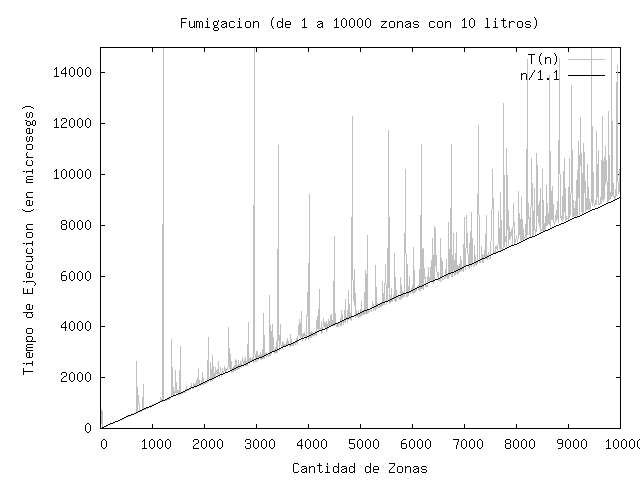
\includegraphics[width=0.7\textwidth]{Plots/Tp2Ej1-TiemposFumigacionPorZonas-10litros-bw.png}
\begin{center}
Figura 1.1
\end{center}
 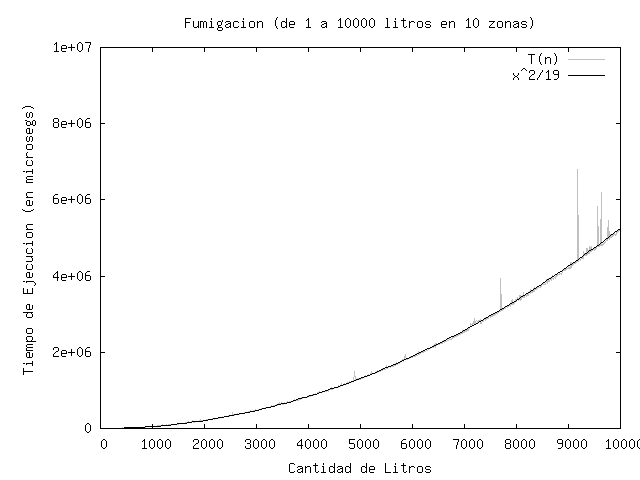
\includegraphics[width=0.7\textwidth]{Plots/Tp2Ej1-TiemposFumigacionPorLitros-10zonas-bw.png}
\begin{center}
Figura 1.2
\end{center}
\end{center}

Ambos gr\'aficos permiten observar algunas cuestiones interesantes. La Figura 1.1 permite observar como el comportamiento del algoritmo de \textit{fumigaci\'on} con respecto a la cantidad de zonas se asimila a una funci\'on lineal, hecho que se corresponde con la complejidad calculada anteriormente. Del mismo modo, la Figura 1.2 muestra como la funci\'on T(n) que representa el tiempo de ejecuci\'on se comporta pr\'acticamente igual que la funci\'on $f(n) = n^2/19 \in O(n^2)$. Este hecho demuestra emp\'iricamente que la complejidad con respecto a la cantidad de litros es cuadr\'atica al realizar la fumigaci\'on tal como se hab\'ia analizado anteriormente.

Otras cuesti\'on observable son los ``picos'' y variaciones abrutas en ambos gr\'aficos. En principio, esto no deber\'ia ocurrir ya que la complejidad no depende de la forma de la entrada como se mencion\'o anteriormente. El motivo de esto radica simplemente en los errores de precisi\'on en la medici\'on de las operaciones propios de las limitaciones de la m\'aquina de c\'omputo utilizada. Los tiempos de ejecuci\'on del algoritmo son mucho mayores en la Figura 1.2 lo que resulta en una mayor estabilidad en los c\'alculo de tiempo, en contraste con la Figura 1.1 donde hay mayor impresici\'on porque dicho gr\'afico refleja cambios de valores m\'as abrutos.

\begin{center}
 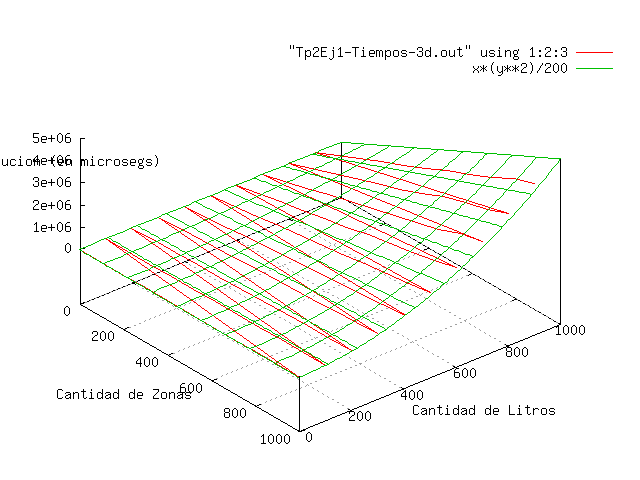
\includegraphics[width=0.7\textwidth]{Plots/Tp2Ej1-TiemposFumigacion-3d-bw.png}
\begin{center}
Figura 1.3
\end{center}
\end{center}

Esta \'ultima figura permite ver como el algoritmo en su totalidad realmente se comporta de la forma esperada. 
Para esto basta comparar los tiempos de ejecuci\'on al variar ambos par\'ametros (litros y zonas) junto con la funci\'on $f(n,m) = n*m^2/200 \in O(n*m^2)$ viendo que ambas ``mantas'' coiniciden. Este ultimo hecho constituye la \'ultima prueba de que empir\'icamente el algoritmo funciona tal como se esperaba.

\subsection*{C\'alculo de Litros Por Zona}

En esta secci\'on analizaremos el comportamiento del otro algortimo propuesto que se encarga de dar parte de la soluci\'on del problema: el algoritmo encargado de calcular los litros a utilizar por cada zona. Los siguientes gr\'aficos muestran el comportamiento del mismo en base a las dos variables en cuesti\'on de forma independiente:

\begin{center}
 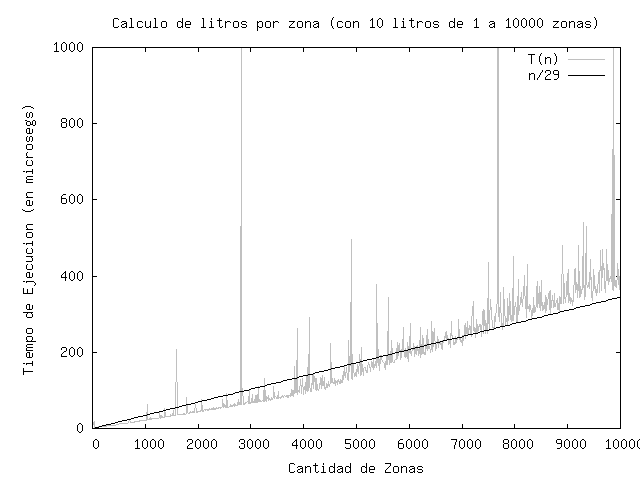
\includegraphics[width=0.7\textwidth]{Plots/Tp2Ej1-TiemposLitrosPorZonaPorZonas-10litros-bw.png}
\begin{center}
Figura 2.1
\end{center}
 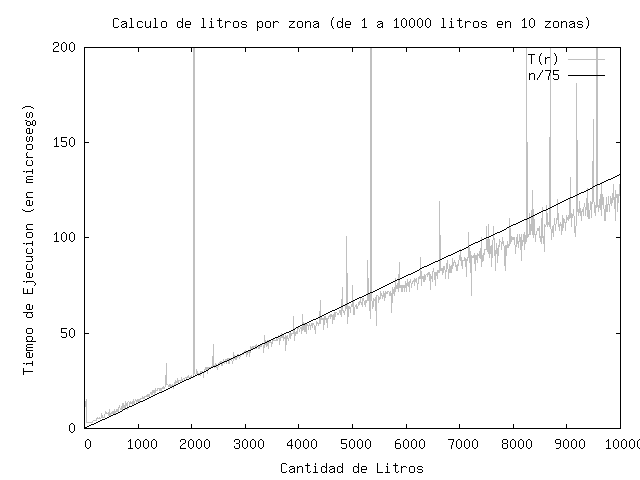
\includegraphics[width=0.7\textwidth]{Plots/Tp2Ej1-TiemposLitrosPorZonaPorZonas-10zonas-bw.png}
\begin{center}
Figura 2.2
\end{center}
\end{center}

Como se puede observar, en ambos casos, el comportamiento del algoritmo es el esperado. La Figura 2.1 muestra como el c\'alculo de litros por zona se ``corresponde'' con el gr\'afico de la funci\'on lineal $f(n) = n/25$ al variar la cantidad de zonas y fijar los litros en $10$. As\'imismo, la Figura 2.2 se comporta de la forma $f(n) = n/75$ al variar los litros y fijar las zonas. Esto comprueba la linealidad en complejidad te\'orica analizada previamente para ambas variables. Un punto interesante a observar es que las constantes que acompañan a estas funciones difieren, siendo la constante relacionada al primer gr\'afico ($1/25$) 3 veces mayor que la otra ($1/75$). Al tratarse de instancias de igual tamaño (en ambos casos, matrices desde $1*10$ hasta $10000*10$), se puede concluir que la \textit{performance} de este algoritmo depende en mayor medida de la cantidad de zonas que de la cantidad de litros. En otras palabras, para instancias de igual tamaño, un caso demora 3 veces m\'as el otro. \textbf{POR QUE?}

Con respecto a la irregularidad del gr\'afico, cabe notar que, a diferencia del algoritmo anterior, este algoritmo no realiza siempre la misma cantidad de operaciones para instancias de igual tamaño tal como se vi\'o en la secci\'on de an\'alisis de complejidad, ya que el recorrido inverso de la matriz resultante depende justamente de los valores que esta contenga que dependen a su vez de los valores de la matriz de entrada \textit{mosquitosMuertos} (ver secci\'on \textit{Algoritmo}). Por este motivo, debido a que se trata de instancias aleatorias, es esperable que no se obtenga un comportamiento ``tan'' similar a la funci\'on lineal propuesta como ocurre para el primer algoritmo.

Por \'ultimo, al igual que para el algoritmo anterior, se presenta el siguiente gr\'afico de 3 dimensiones:

% \begin{center}
%  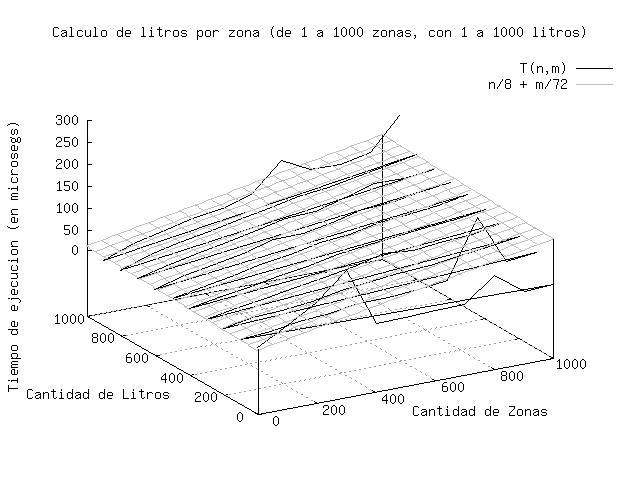
\includegraphics[width=0.7\textwidth]{Plots/Tp2Ej1-TiemposLitrosPorZona-3d-bw.png}
\begin{center}
Figura 1.3
\end{center}
% \end{center}

Al igual que antes, este gr\'afico permite ver la complejidad de ambos par\'ametros en conjunto. \textbf{TODO}

\section*{Conclusiones}

%TODO: Decir que se podria haber analizado los algoritmos recursivos que repiten operaciones vs la programacion dinamica pero no hubo tiempo.

% Este ejercicio nos mostr\'o un caso representativo en el que el tiempo de ejecuci\'on difiere notablemente a la complejidad calculada para el peor caso.
% 
% Para este algoritmo en particular se debe a que la funci\'on \textit{encontrarPrimos} alcanzar\'ia dicho peor caso si la conjetura de Goldbach fuese falsa, cuesti\'on que no sucede para ning\'un n\'umero que pueda tomar la func\'on (es decir, hasta el n\'umero mas grande almacenable en un \textit{int}). M\'as aun, esta demostrado que para n\'umeros mucho mas grandes que los testeados la conjetura se sigue cumpliendo (ver secci\'on Referencias para m\'as detalles) por lo que en el \'ambito cient\'ifico se cree que es cierta.
% 
% Tambi\'en vimos casos en los que entre n\'umeros cercanos tomados por la funci\'on, el tiempo de ejecuci\'on difiere considerablemente. Adem\'as notamos que a medida que el tama\~{n}o del par\'ametro de entrada crece el tiempo tamb\'ien lo hace, pero siempre muy lejos de los peores casos para dichas entradas. Estas situaciones se deben a la desconocida distribuci\'on de los n\'umeros primos entre los naturales, por lo que no podemos dar una explicaci\'on general que incluya todos los casos reales. Sin embargo, en base a todos los an\'alisis realizados, podemos concluir que para todos los casos computables por nuestro algoritmo el tiempo de ejecuci\'on ser\'a mas que aceptable.

TODO

\bigskip

\begin{center}
\section*{Ejercicio 2: Encontrar Diamante en un grafo}
\end{center}

\bigskip
\section*{Introducci\'on}

El objetivo del siguiente ejercicio es dise\~{n}ar un algoritmo que, dado un grafo, encuentre el menor subgrafo inducido isomorfo a un diamante, en caso de que \'este exista. Un diamante puede definirse como un grafo $K_{4}$ menos una arista. Este algoritmo est\'a basado en una propiedad sobre diamantes (enunciada en el Anexo A) que, adem\'as de ser usada para resolver el problema, ser\'a demostrada de manera formal.

En un principio, cuando se comenz\'o a idear el algoritmo, surgi\'o la idea de utilizar solamente la propiedad enunciada para resolver el problema. Es decir, para toda vecindad de cada nodo, estudiar cada componente conexa para determinar si la misma es completa. Sin embargo, esto s\'olo aportaba informaci\'on sobre las componentes conexas que formaban un diamante, pero no brindaba detalles sobre los nodos que formaban el diamante, y no aseguraba que este fuera m\'inimo para dicha componente conexa. Por esta raz\'on, se opt\'o por utilizar un m\'etodo m\'as complejo que, aunque se basa en la propiedad mencionada, obtiene de cada componente conexa no completa (existe diamante) los nodos m\'inimos que forman un diamante. Esto se realiza calculando el m\'inimo nodo que puede formar un diamante y, a partir de este, construir el m\'inimo probando las posibles combinaciones que construyan un diamante. De esta manera se pueden obtener los diamantes m\'inimos de cada componente conexa no completa de una determinada vecindad y as\'i determinar el m\'inimo de la misma. Finalmente, se comparan los diamantes obtenidos de cada vecindad para obtener el m\'inimo diamante del grafo. Este algoritmo ser\'a explicado en detalle, se mostrar\'a su correctitud y se presentar\'a la implementaci\'on y pruebas de ejecuci\'on del mismo en posteriores secciones.

\section*{Demostraci\'on de la parte a}

A continuaci\'on se presentar\'a la demostraci\'on de la siguiente propiedad:

Sea $G$ un grafo de $n$ v\'ertices y $m$ aristas, $G$ no contiene un subgrafo diamante como subgrafo inducido si y solamente si para todo v\'ertice $v$, su vecindad $N(v)$ se divide en componentes conexas completas.

Llamaremos $p$ a la proposici\'on ``$G$ no contiene un subgrafo diamante como subgrafo inducido`` y $q$ a la proposici\'on ''para todo v\'ertice $v$, su vecindad $N(v)$ se divide en componentes conexas completas``. Dividiremos la demostraci\'on en dos partes: la implicaci\'on y la vuelta.

\begin{itemize}
\item $p \Longrightarrow q$

Por propiedades de la l\'ogica $p \Longrightarrow q$ equivale a mostrar $-q \Longrightarrow -p$. De esta manera, probaremos aqu\'i que si existe un v\'ertice $v$ tal que su vecindad $N(v)$ contiene una componente conexa no completa entonces $G$ contiene un subgrafo diamante como subgrafo inducido.

Primero probaremos la siguiente propiedad (propiedad 1): Sea $v$ un v\'ertice de $G$ y sea $N(v)$ su vecindad asociada. Si $N(v)$ tiene a $K_{3}$ menos una arista (lo llamaremos $K_{3}-1$) como subgrafo inducido, entonces $G$ contiene un diamante como subgrafo inducido.

Esto se debe a que, al pertenecer $K_{3}-1$ a la vecindad de $v$, el grafo original contiene a $K_{3}-1$ uniendo todos sus vertices con $v$, esto implica agregarle un nodo ($v$) y tres aristas (ya que $v$ es adyacente a los tres nodos que conforman el $K_{3}-1$ porque pertenecen a su vecindad). Como $K_{3}-1$ tiene dos aristas entonces agregando un nodo y sumando tres aristas tengo un $K_{4}-1$ (definici\'on de diamante).

Viendo esto, basta probar que si existe un v\'ertice $v$ tal que su vecindad $N(v)$ tiene una componente conexa no completa entonces dicha componente contiene un $K_{3}-1$. Para esto, mostraremos ahora que todo grafo $G$ conexo y no completo contiene un $K_{3}-1$ (propiedad 2).

Como $G$ no es completo pero si conexo, existen dos nodos $a$ y $z$ tal que no son adyacentes y existe un camino entre ellos. Sea $b$ un nodo adyacente a $a$ que pertenece al camino entre $a$ y $z$. $b$ es distinto de $z$ ya que si fueran iguales $a$ y $z$ ser\'ian adyacentes y eso es absurdo por hipotesis. Ahora tomamos un nodo adyacente a $b$ que tambi\'en pertenezca al camino entre $a$ y $z$ al que llamaremos $c$. Este nodo puede ser igual a $z$ (en caso de que el camino tenga longitud dos) o un nodo intermedio en el camino entre $a$ y $z$. Si $c$ es igual a $z$ entonces me puedo formar un $K_{3}-1$ ya que $a$ es adyacente a $b$, $b$ es adyacente a $z$ y $z$ no es adyacente a $a$ por hipotesis:
\begin{center}
 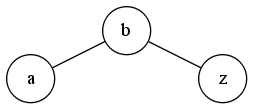
\includegraphics[width=0.34\textwidth]{Grafos/ej2figura1-1.png}
\end{center}
Si $c$ es distinto de $z$ entonces tenemos dos casos: si $c$ no es adyacente a $a$ entonces podemos formar un $K_{3}-1$ con dichos nodos:
\begin{center}
 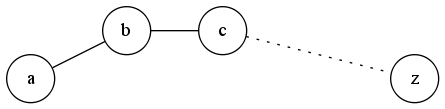
\includegraphics[width=0.6\textwidth]{Grafos/ej2figura1-2.png}
\end{center}
Si $c$ si es adyacente a $a$, entonces no podemos formar un $K_{3}-1$ entre $a$ $b$ y $c$:
\begin{center}
 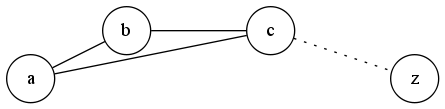
\includegraphics[width=0.6\textwidth]{Grafos/ej2figura1-3.png}
\end{center}
En este \'ultimo caso tomamos como nuevo nodo $b$ a $c$ (es adyacente a $a$ y pertenece al camino entre $a$ y $z$) y como nuevo nodo $c$ a un nodo adyacente a $c$ que pertenezca al camino entre $a$ y $z$ y todavia no haya sido recorrido (siguiendo el orden alfabetico seria el nodo $d$). Nuevamente caemos en el caso anterior, donde la posibilidad de poder armar un $K_{3}-1$ depende de si $d$ es adyacente o no a $a$. Si no es posible obtener un $K_{3}-1$ con el nodo $d$ (debido a que $d$ es adyacente a $a$), seguiremos avanzando los dos nodos pertenecientes al camino entre $a$ y $z$ hasta llegar a que el primero de los dos es el nodo anterior a $z$ (lo llamaremos $y$) del camino y el segundo nodo es igual a $z$. En este caso, siempre es posible armar un $K_{3}-1$ ya que $z$ no es adyacente a $a$ por hipotesis:
\begin{center}
 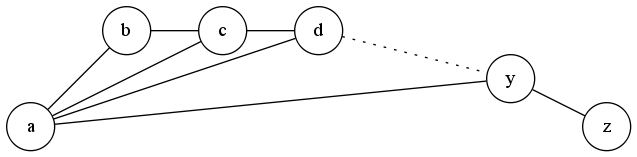
\includegraphics[width=0.85\textwidth]{Grafos/ej2figura1-4.png}
\end{center}
Finalmente hemos probado que si existe un v\'ertice $v$ de $G$ tal que su vecindad $N(v)$ tiene una componente conexa no completa entonces dicha componente contiene un $K_{3}-1$ (por 2), y esto implica que $G$ contiene un subgrafo diamante como subgrafo inducido (por 1).

\item $q \Longrightarrow p$

Por propiedades de la l\'ogica $q \Longrightarrow p$ equivale a mostrar $-p \Longrightarrow -q$. De esta manera, probaremos aqu\'i que si $G$ contiene un subgrafo diamante como subgrafo inducido entonces existe un v\'ertice $v$ tal que su vecindad $N(v)$ contiene una componente conexa no completa.

Sea $G$ un grafo que contiene un subgrafo diamante como subgrafo inducido. Sea $G_{D}$ el subgrafo diamante de $G$:
\begin{center}
 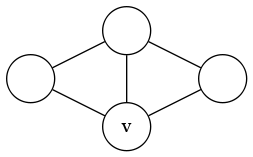
\includegraphics[width=0.34\textwidth]{Grafos/ej2figura2-1.png}
\end{center}
Si tomo uno de los dos nodos de $G_{D}$ de grado tres, que llamaremos $v$, su vecindad $N_{G_{D}}(v)$ sera:
\begin{center}
 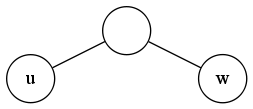
\includegraphics[width=0.34\textwidth]{Grafos/ej2figura2-2.png}
\end{center}
Podemos ver entonces que $N_{G_{D}}(v)$ tiene una \'unica componente conexa y esta no es completa ya que los dos nodos de grado dos del diamante (en la figura llamados $u$ y $w$) no son adyacentes.

Sea $v$ uno de los dos nodos de grado tres del subgrafo diamante de $G$ y $u$ y $w$ los dos nodos de grado dos de dicho diamante. Si tomo la vecindad $N(v)$ de $v$, como $u$ y $w$ son adyacentes a $v$ (pertenecen al diamante) entonces pertenecen a $N(v)$. Ademas como $u$ y $w$ son los nodos de grado dos del subgrafo diamante entonces no son adyacentes en $G$. Como $u$ y $w$ no son adyacentes en $G$ tampoco lo ser\'an para ningun subgrafo inducido de $G$, en particular para $N(v)$. De esta manera la componente conexa de $N(v)$ que contiene al diamante no es completa.

Concluimos entonces que la propiedad es cierta ya que existe un $v$ para el cual se cumple.

\end{itemize}


\section*{Algoritmo}

% \begin{graph}(4,4)(-2,0)
%  \roundnode{Nodo1}(1,1)
%  \roundnode{Nodo2}(2,2)
%  \edge{Nodo1}{Nodo2}
% \end{graph}
% \originalTeX
% \begin{figure}[htbp]
% 
% \begin{graph}(4,4)(-2,0)
%   \squarenode{Sq}(-1.5,3.5)
%   \textnode{Te}(1.5,3.5){abc}
%   \roundnode{Ro}(0,.5)
%   \diredge{Sq}{Te}
%   \edge{Sq}{Ro} \diredge{Ro}{Te}
%   \dirbow{Ro}{Sq}{-.2}
%   \dirbow{Ro}{Te}{.2}
%   \dirloopedge{Ro}(-.8,-.2)(-1.2,.4)
%   \dirloopedge{Ro}(.8,-.2)(1.2,.4)
%   \loopedge{Ro}{15}(0,-.5)
% \end{graph}
% % \germanTeX
% \end{figure}


A continuaci\'on se presenta el pseudoc\'odigo del algoritmo para resolver el problema propuesto.

\begin{verbatim}
leer archivo y crear adyacencias excepto para los nodos de grado 1 y 0,
un arreglo donde cada posicion i es una lista de los nodos adyacentes del nodo i

Armar la matriz de adyacencias

para cada nodo (que llamaremos superNodo) del grafo
  si el tamaño de la lista de adyacencia de superNodo es mayor que 3
    vecindadDeSuperNodo = crearVecindad(superNodo)
    agregar buscarDiamanteMinimoEnVecindad(vecindadDeSuperNodo) a diamantesMinimos

diamanteMinimo = minimo(diamantesMinimos)
guardar en "Tp2Ej2.out" diamanteMinimo


crearVecindad(superNodo) { 
  para cada nodo k de adyacencias[superNodo]
    para cada nodo j de adyacencias[k]
      si nodo j es adyacente a superNodo
        agregar nodo j a listaVecindad
    vecindadDeSuperNodo[k] = listaVecindad
  devolver vecindadDeSuperNodo //esto es un grafo (array de listas de adyacencia)
}

buscarDiamanteMinimoEnVecindad(vecindadDeSuperNodo) { 
  Recorrer una componente conexa (no recorrida previamente) de vecindadDeSuperNodo por DFS 
  sumando los grados de los nodos recorridos (sumaGradosCompConexa) y
  guardando en nodosCompConexa los nodos recorridos y
  en nodoMinimoCompConexa el nodo minimo de la componente conexa
  
  si sumaGradosCompConexa != cant de nodos de un grafo completo de tam(nodosCompConexa) nodos
    si diamanteMinimo no existe o nodoMinimoCompConexa <= minimo(diamanteMinimo)
      diamante = buscarDiamanteMinimoDeCompConexa(superNodo,vecindadDeSuperNodo,nodosCompConexa)
      si diamanteMinimo no existe o si existe y es mas grande que diamante
        diamanteMinimo = diamante

  devolver diamanteMinimo //si es null es porq no habia diamante en toda la vecindad
}

buscarDiamanteMinimoDeCompConexa(superNodo, vecindadDeSuperNodo, nodosCompConexa) {
  nodo1 = superNodo
  nodoMinimo = nodo minimo de nodosCompConexa con grado menor que tam(nodosCompConexa)-1

  para cada nodo (adyacenteANodo2) de vecindadDeSuperNodo[nodo2] //O(tam(nodosCompConexa))
    para cada nodo (nodoCandidato) de vecindadDeSuperNodo[adyacenteANodo2]
      si nodoCandidato no es adyacente a nodo2 y <nodoCandidato, adyacenteANodo2> < tuplaMin
        tuplaMin = <nodoCandidato, adyacenteANodo2>

  nodo3 = primero(tuplaMin)
  nodo4 = segundo(tuplaMin)

  diamanteMinimo = ordenar(nodo1, nodo2, nodo3, nodo4)

  devuelvo diamanteMinimo
}

\end{verbatim}

Como se mencion\'o anteriormente, este algoritmo est\'a basado en la propiedad demostrada en el punto a, es decir, para cada nodo del grafo estudia las componentes conexas de la vecindad de dicho nodo para determinar si existe un diamante. En primer lugar, se eliminan todos los nodos de grado 0 \'o 1, ya que estos no pueden formar parte de ning\'un diamante y eliminarlos no afecta a ning\'un diamante del grafo. Esto se debe a que cualquier nodo que pertenezca a un diamante tiene por lo menos grado 2. En segundo lugar, se crean la lista de adyacencias (que llamaremos \textit{adyacencias}) y la matriz de adyacencia, que resultar\'an necesarias para calcular la vecindad de cada nodo y verificar si dos nodos son adyacentes, respectivamente. Luego, el algoritmo comienza a chequear por cada nodo (en adelante llamaremos superNodo) su vecindad para encontrar componentes conexas no completas y as\'i determinar donde se encuentra el diamante. La funci\'on \textit{crearVecindad} se encarga de construir la vecindad (que es un grafo representado con una lista de adyacencia) de cada superNodo a partir de la lista \textit{adyacencias}, es decir, por cada elemento k de la lista de adyacencia de superNodo se recorre la lista de adyacencia del elemento k agregando en la vecindad los elementos que est\'an relacionados con superNodo.

Una vez obtenida la vecindad (vecindadDeSuperNodo), se comienza a revisar las componentes conexas de la misma para verificar si son completas a trav\'es de la funci\'on \textit{buscarDiamanteMinimoEnVecindad}. Con este fin, se utiliza Depth First Search (DFS) para recorrer cada componente conexa almacenando la suma de los grados de cada nodo recorrido as\'i como el nodo m\'inimo encontrado (nodoMinimoCompConexa) y la lista de nodos por los que se avanz\'o (nodosCompConexa). Al terminar de recorrer cada componente conexa, se verifica si la misma es completa o no. En caso de que no lo sea, se sabe que ninguno de los nodos de esa componente conexa forma un diamante\footnotemark[1], por lo que se descarta y contin\'ua verificando las siguientes componentes. En caso afirmativo, se procede a encontrar los nodos que forman el diamante\footnotemark[1] m\'inimo para esa componente conexa por medio de la funci\'on \textit{buscarDiamanteMinimoDeCompConexa}. Esta funci\'on utiliza el nodo m\'inimo de la componente conexa (nodoMinimoCompConexa) recorrida para obtener el diamante. Es decir, toma la lista de adyacencia de nodoMinimoCompConexa y para cada nodo k de dicha lista, recorre todos los elementos j de su lista de adyacencia para determinar si forma un $K_{3}-1$ entre nodoMinimoCompConexa, $k$ y $j$. En este caso, se sabe que los elementos encontrados forman un diamante con superNodo, ya que superNodo es adyacente a los mismos pues pertenecen a su vecindad. Como la funci\'on \textit{buscarDiamanteMinimoDeCompConexa} verifica en cada paso si el diamante obtenido es menor al que se tiene hasta ese momento y se prueban todas las posibles diamantes constru\'idos a partir de nodoMinimoCompConexa, se puede afirmar que obtiene el diamante m\'inimo para dicha componente conexa. Esto se debe a que nodoMinimoCompConexa es el menor nodo que puede formar un diamante\footnotemark[1] y los restantes nodos se obtienen seleccionando el menor de todos los posibles diamantes.

Luego, dentro de la funci\'on \textit{buscarDiamanteMinimoEnVecindad} se verifica si el diamante m\'inimo de la componente conexa actual es menor que el diamante que se tiene hasta ese paso (almacenado en diamanteMinimo). Si esto sucede, el diamante de la componente conexa actual pasa a ser el diamante m\'inimo. Una vez verificadas todas las componentes conexas se obtiene, en diamanteMinimo, el m\'inimo diamante para la vecindad de superNodo. Este diamante se almacena en una lista llamada diamantesMinimos que, cuando el algoritmo termina de verificar las vecindades de todos los nodos, contendr\'a los diamantes m\'inimos para cada una de las mismas, en caso de que este exista. Finalmente, se busca el m\'inimo de la lista diamantesMinimos, con lo que se obtiene el diamante m\'inimo de todo el grafo, resolviendo as\'i el problema.

\footnotetext[1]{Las demostraciones de estas propiedades fueron presentadas en la secci\'on ``Demostraci\'on de la parte a''}

\section*{Complejidad}

Como el algoritmo propuesto se basa en la t\'ecnica de \textit{backtracking}, la complejidad del mismo en el peor caso es similar a la de un algoritmo de fuerza bruta. En este tipo de algoritmos, se generan todas las soluciones posibles y se eval\'uan para determinar si cumplen con el problema a resolver. La complejidad de generar y revisar todas las soluciones posibles es exponencial y, en particular, el algoritmo de fuerza bruta aplicado al problema presentado ser\'ia $O(n!)$, con $n$ la cantidad de fichas del tablero. A pesar de que los algoritmos de \textit{backtracking} descartan gran cantidad de casos y aplican podas para reducir el tiempo de ejecuci\'on, existen casos patol\'ogicos en que pocas de estas optimizaciones pueden ser utilizadas y, por lo tanto, se recorran todas las ramas de soluciones. Estos casos hacen que la complejidad en el peor caso del algoritmo presentado sea la misma que la de un algoritmo de fuerza bruta, es decir $O(n!)$ (siendo $n$ la cantidad de fichas totales del tablero). Sin embargo, como estudiaremos en posteriores secciones, el tiempo de ejecuci\'on del algoritmo difiere significativamente del tiempo del algoritmo de fuerza bruta.

\section*{An\'alisis de resultados}

En la presente secci\'on se mostrar\'an los an\'alisis realizados para grafos con distinta cantidad de nodos. El enfoque principal de las pruebas radica en estudiar los tiempos de ejecuci\'on del algoritmo para casos aleatorios y estudiar el comportamiento para los peores casos. Con este fin se implement\'o un algoritmo que genera grafos aleatorios de $n$ cantidad de nodos, siendo $n$ el par\'ametro de dicha funci\'on. De esta manera, utilizando dicho algoritmo para distintos valores de $n$, se contrastaron los tiempos de ejecuci\'on con la cota estudiada. Como se mencion\'o en la secci\'on anterior, la complejidad del algoritmo es $O(n*m)$ pero a fin de estudiar los resultados acotaremos esta complejidad a $O(n^{3})$ ya que en cualquier grafo la cantidad de aristas $m$ est\'a acotada por $n*(n-1)/2$ es decir, $m$ es del orden de $n^{2}$. Esta acotaci\'on aporta simplicidad al estudio de resultados, sin embargo, como el algoritmo tiene una cota menor se espera que los tiempos de ejecuci\'on tengan un crecimiento menor que c\'ubico (en relaci\'on a la cantidad de nodos).

La primera prueba realizada consisti\'o en generar grafos aleatorios variando su cantidad de nodos entre $1$ y $500$. Para cada grafo se estudi\'o su tiempo de ejecuci\'on y a continuaci\'on se presentan los resultados obtenidos.

\begin{center}
 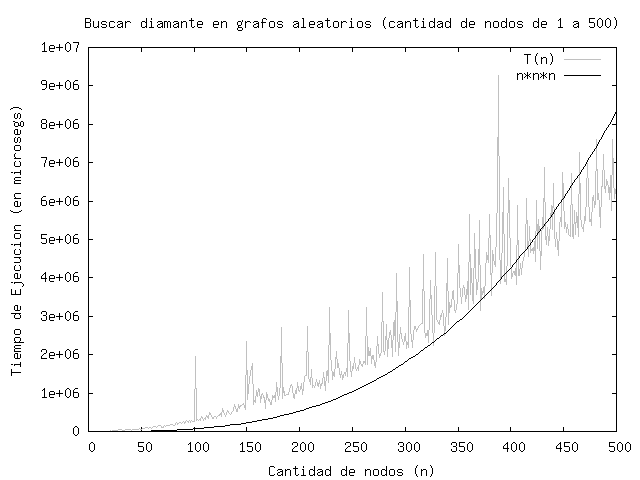
\includegraphics[width=0.7\textwidth]{Plots/Tp2Ej2-Complejidad.png}
\begin{center}
Figura 2.1
\end{center}
\end{center}

Como se puede apreciar en el gr\'afico, el crecimiento de los tiempos de ejecuci\'on del algoritmo es ligeramente inferior a la cota te\'orica propuesta. Como se mencion\'o anteriormente, esto se corresponde con lo esperado, ya que para este an\'alisis de utiliz\'o una cota mayor a la del algoritmo ($O(n^{3})$). Adem\'as se pueden apreciar irregularidades en la curva obtenida, lo que indica que el tiempo que se tarda en encontrar un diamante en un determinado grafo, adem\'as de depender de la cantidad de nodos, est\'a determinado por la disposici\'on de las aristas del mismo. Es decir, por la forma en la que est\'a hecho el algoritmo, el tiempo de ejecuci\'on va a depender de la cantidad de componentes conexas en las que tenga que buscar el diamante m\'inimo, para cada vecindad de cada nodo. Los peores casos se dar\'an en grafos en los que se busque un diamante en la mayor\'ia de las componentes conexas de cada vecindad. Estos casos hacen que las optimizaciones del algoritmo, que descartan la b\'usqueda de un diamante m\'inimo en ciertas componentes conexas, sean ineficientes. 

A continuaci\'on presentaremos alguno de estos casos ``patol\'ogicos'' y se ver\'a por qu\'e no se aplican las optimizaciones.

\begin{center}
 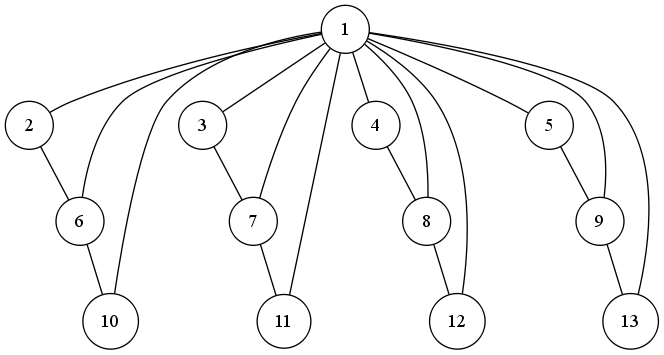
\includegraphics[width=0.7\textwidth]{Grafos/grafomati.png}
\begin{center}
Figura 2.2
\end{center}
\end{center}

Como se puede observar en el grafo presentado, la vecindad del nodo $1$ tiene varias componentes conexas que forman un diamante, ya que ninguna es completa. Por esta raz\'on, se deben estudiar todas las componentes conexas para encontrar el diamante m\'inimo. Sin embargo, podr\'ia darse el caso en que el algoritmo implementado no tenga que buscar el diamante m\'inimo para todas debido a que el m\'inimo nodo de una componente conexa (llamado nodoMinimoCompConexa en la secci\'on algoritmo) es menor que el m\'inimo nodo de las otras componentes. Esto suceder\'ia, por ejemplo, si el algoritmo comenzara a estudiar la componente conexa que comienza con el nodo $2$. Por el contrario, en el caso en que comenzara por la componente conexa que tiene el nodo $5$ y recorriera de derecha a izquierda las componentes conexas del gr\'afico, se tendr\'ia que calcular el m\'inimo diamante para todas las componentes, por lo que la cantidad de operaciones ser\'ia mayor. La forma en que se recorren las componentes conexas depende exclusivamente del orden de las listas de adyacencias pasadas como par\'ametro, por lo que la aparici\'on de estos peores casos estar\'a ligada a esta distribuci\'on. 

Cabe aclarar que el esquema presentado en la figura 2.2 representa s\'olo un caso simplificado sobre los peores casos que se pueden encontrar para el algoritmo mencionado. Es decir, en este gr\'afico s\'olo la vecindad del nodo $1$ podr\'ia representar un peor caso. F\'acilmente, este gr\'afico podr\'ia extenderse para formar casos a\'un peores, ya que cualquiera de las vecindades de los otros nodos podr\'ia tener las mismas dificultades que las del nodo $1$. Como los peores casos dependen del orden en que se reciben las listas de adyacencias, se hace dificultosa la b\'usqueda de los mismos. Por esta raz\'on, se opt\'o por explicar en detalle que representar\'ia un peor caso, ya que encontrar y hacer preubas de tiempo de ejecuci\'on sobre los mismos resultaba una tarea muy compleja.

\section*{Conclusiones}

A lo largo del desarrollo del ejercicio, se experimentaron las particularidades de un algoritmo de \textit{backtracking}. Nos encontramos con diversas dificultades en la implementaci\'on, a pesar de que la idea intuitiva del algoritmo es relativamente simple. Adem\'as, llegamos a la conclusi\'on de que, si bien la complejidad en peor caso es muy elevada, el algoritmo en general suele ser mucho m\'as eficiente que algoritmos que utilizan la t\'ecnica de fuerza bruta para resolver este tipo de problemas. 

Los principales incovenientes que surgen al implementar un algoritmo de \textit{backtracking} tienen que ver con la elecci\'on de la poda. Al momento de dicha elecci\'on, se deben considerar los aspectos de eficiencia, dificultad en la implementaci\'on y sobre todo, los beneficios (en relaci\'on al tiempo de ejecuci\'on) que esta provocar\'ia. Al pensar en detalle cada uno de las posibles podas, estos factores fueron determinantes para tomar una decisi\'on; podas que parec\'ian muy eficientes en principio, resultaban muy dif\'iciles de implementar y no aportaban cambios significativos que justifiquen su uso. A su vez, podas que parec\'ian descartar muchos casos, terminaban empeorando el tiempo de ejecuci\'on.

Es importante destacar que al aplicar la poda propuesta, el algoritmo mejora considerablemente en promedio. Esta situaci\'on resultaba esperable y pudo ser comprobada emp\'iricamente en las pruebas realizadas. Tambi\'en, se not\'o una relaci\'on entre la distribuci\'on de fichas de entrada y el tiempo de ejecuci\'on del algoritmo presentado. Por ejemplo, existen casos en los que la disposici\'on de las fichas no permitan hacer podas y otros en los que no sea necesario tener que reemplazar alguna ficha.

En conclusi\'on, la eficiencia del algoritmo de \textit{backtracking} depende fuertemente de las podas que se realicen y de la distribuci\'on probabil\'istica de los par\'ametros de entrada para casos promedio. Por esta raz\'on, la implementaci\'on de podas es determinante y justifica el tiempo invertido en idear las mismas.

\begin{center}
\section*{Ejercicio 3: C\'alculo de la mediana entre dos vectores}
\end{center}

\bigskip
\section*{Introducci\'on}

El problema que plantea este ejercicio es calcular la mediana entre dos vectores de n\'umeros enteros, es decir, el elemento que, una vez concatenados y ordenados los vectores, deja a ambos lados la misma cantidad de elementos. Seg\'un lo especificado en el problema, ambos vectores tienen la misma longitud y est\'an ordenados.

En principio, la soluci\'on trivial del problema fue descartada ya que el costo de realizarla era excesivo para los fines del ejercicio. Esta soluci\'on consist\'ia en concatenar ambos vectores, ordenarlos y posteriormente obtener la mediana a partir del elemento medio de dicha secuencia.

Descartada esta opci\'on, surgi\'o la idea de desechar una gran cantidad de elementos, cuando sea posible, para poder realizar los c\'alculos sobre una cantidad de n\'umeros considerablemente inferior a la inicial. De esta manera, la complejidad resultar\'ia del costo de descartar los elementos apropiados y luego hacer el c\'alculo con una cantidad peque\~{n}a de elementos. Evidentemente, nuestro algoritmo seguir\'ia el concepto de Divide and Conquer cl\'asico.

Con las ideas m\'as claras, notamos que descartando la misma cantidad de elementos mayores o iguales a la mediana, que menores o iguales a ella, \'esta se manten\'ia como valor medio de los vectores generados a partir de los elementos no descartados. R\'apidamente, nos dimos cuenta que la mediana de concatenar dos vectores ordenados, se encuentra entre los elementos mayores a la mediana del vector con menor valor medio y los elementos menores a la mediana del vector con mayor valor medio (conjetura que luego se demostrar\'a).

Planteado todo esto, result\'o sencillo escribir el pseudoc\'odigo de nuestro algoritmo. 

\section*{Algoritmo}

A continuaci\'on se mostrar\'a el pseudoc\'odigo del algoritmo implementado seguido de una demostraci\'on de su correctitud.

\begin{verbatim}
medianaRecursiva (vector x[0..n-1], vector y[0..n-1])

  si n == 1
    si x[0] > y[0]
      devolver y[0]
    sino
      devolver x[0]

  si n == 2
    si x[0] == y[0]
      devolver x[0]
    si x[0] > y[0]
      si x[0] > y[1]
        devolver y[1]
      sino
        devolver x[0]
    sino
      si x[1] > y[0]
        devolver y[0]
      sino
        devolver x[1]

  si n > 2
    si n es impar
      medio = n / 2
    sino
      medio = n / 2 - 1;
    si x[medio] > y[n/2]
      devolver medianaRecursiva(x[0..medio], y[n/2..n-1]);
    sino
      devolver medianaRecursiva(x[medio..n-1], y[0..n/2]);
\end{verbatim}

Con respecto a la implementaci\'on del algoritmo, la misma result\'o bastante sencilla de realizar en el lenguaje C++, utilizando las operaciones b\'asicas que provee el lenguaje y usando arreglos b\'asicos para la reprentaci\'on de los vectores. La \'unica parte no trivial radica en el uso de punteros para lograr llamar recursivamente a la func\'on con las ``mitades'' correspondientes de cada arreglo. Tambi\'en, cabe notar que en la implementaci\'on fue necesario pasar como par\'ametro extra el tama\~{n}o de los arreglos que reprentan a los vectores por cuestiones intr\'insicas al manejo de arreglos din\'amicos en C++.

Como se puede apreciar, el algoritmo sigue los pasos de un algoritmo cl\'asico de \textit{divide and conquer} dividiendo el problema en arreglos de menor tama\~{n}o al ir descartando elementos mayores y menores a la mediana. De esta manera, si logramos mostrar que en cada llamado recursivo la mediana original es la misma que la de los dos nuevos arreglos, entonces podremos asegurar que el algoritmo es correcto. Para mostrar esto primero veremos que en cada paso la mediana sigue estando dentro de alguno de los arreglos, y luego que los n\'umeros menores o iguales a la mediana descartados son la misma cantidad que los n\'umeros mayores o iguales a la misma que se descartan.

\subsection*{Demostraci\'on de que la mediana se encuentra en el pr\'oximo llamado recursivo}

Dividiremos la demostraci\'on en dos casos, cuando la longitud de los arreglos iniciales es impar y cuando es par.

Sean $X$ e $Y$ los arreglos iniciales, entonces si llamo $A$ a $concatenar(X,Y)$ tengo que $ordenar(A)=[a_{1},a_{2},..,a_{n},..,a_{2n}]$, como la longitud de $A$ es par, su mediana es $a_{n}$. Se puede ver entonces que la mediana tiene $n-1$ elementos menores o iguales a ella ($A[1..n-1]$) y n elementos mayores o iguales ($A[n+1..2n]$).

\begin{enumerate}
 \item Longitud impar:
  
Los arreglos que tomar\'a la funci\'on para el llamado recursivo estan dados por la comparaci\'on entre las medianas de los mismos siendo $x_{(n+1)/2}$ la mediana de $X$ e $y_{(n+1)/2}$ la mediana de $Y$.
\begin{enumerate}
\item $x_{(n+1)/2}\geq y_{(n+1)/2}$:

En este caso el algoritmo toma como nuevos arreglos a $X[1..(n+1)/2]$ e $Y[(n+1)/2..n]$. Supongo ahora, que $m$ (a partir de ahora nos referiremos asi a la mediana) no est\'a en los nuevos arreglos, es decir, pertenece a $X((n+1)/2..n]$ o a $Y[1..(n+1)/2)$.
\begin{enumerate}
\item
 Si $m \in X((n+1)/2..n] \Longrightarrow m \geq x_{(n+1)/2}$. Si $m=x_{(n+1)/2}$ entonces SI pertenece a los nuevos arreglos pues $x_{(n+1)/2}$ pertenece. Si no son iguales entonces $m>x_{(n+1)/2} \Longrightarrow m>x \,\,\forall x \in X[1..(n+1)/2]$. Ademas si $m>x_{(n+1)/2}\geq y_{(n+1)/2} \Longrightarrow m>y \,\,\forall y \in Y[1..(n+1)/2]$. Como $X[1..(n+1)/2]$ y $Y[1..(n+1)/2]$ tienen $(n+1)/2$ elementos cada uno entonces $m$ es mayor a $2((n+1)/2)=n+1$ elementos lo que es absurdo porque la mediana solo puede tener tener $n-1$ elementos menores por lo visto anteriormente.
\item
 Si $m \in Y[1..(n+1)/2) \Longrightarrow m \leq y_{(n+1)/2}$. Si $m=y_{(n+1)/2}$ entonces SI pertenece a los nuevos arreglos pues $y_{(n+1)/2}$ pertenece. Si no son iguales entonces $m<y_{(n+1)/2} \Longrightarrow m<y \,\,\forall y \in Y[(n+1)/2..n]$. Ademas si $m<y_{(n+1)/2}\leq x_{(n+1)/2} \Longrightarrow m<x \,\,\forall x \in X[(n+1)/2..n]$. Como $X[(n+1)/2..n]$ y $Y[(n+1)/2..n]$ tienen $(n+1)/2$ elementos cada uno entonces $m$ es menor a $2((n+1)/2)=n+1$ elementos lo que es absurdo porque la mediana solo puede tener tener $n$ elementos mayores por lo visto anteriormente.
\end{enumerate}

De esta manera queda demostrado que si $n$ es impar y $x_{(n+1)/2}\geq y_{(n+1)/2}$ entonces la mediana pertenece a alguno de los nuevos arreglos pasados como par\'ametro.

\item $x_{(n+1)/2}<y_{(n+1)/2}$:

En este caso el algoritmo toma como nuevos arreglos a $X[(n+1)/2..n]$ e $Y[1..(n+1)/2]$. Supongo ahora, que $m$ no est\'a en los nuevos arreglos, es decir, pertenece a $X[1..(n+1)/2)$ o a $Y((n+1)/2..n]$. 
\begin{enumerate}
\item
 Si $m \in X[1..(n+1)/2) \Longrightarrow m \leq x_{(n+1)/2}$. Si $m=x_{(n+1)/2}$ entonces SI pertenece a los nuevos arreglos pues $x_{(n+1)/2}$ pertenece. Si no son iguales entonces $m<x_{(n+1)/2} \Longrightarrow m<x \,\,\forall x \in X[(n+1)/2..n]$. Ademas si $m<x_{(n+1)/2}< y_{(n+1)/2} \Longrightarrow m<y \,\,\forall y \in Y[(n+1)/2..n]$. Como $X[(n+1)/2..n]$ y $Y[(n+1)/2..n]$ tienen $(n+1)/2$ elementos cada uno entonces $m$ es menor a $2((n+1)/2)=n+1$ elementos lo que es absurdo porque la mediana solo puede tener tener $n-1$ elementos menores por lo visto anteriormente.
\item
 Si $m \in Y((n+1)/2..n] \Longrightarrow m \geq y_{(n+1)/2}$. Si $m=y_{(n+1)/2}$ entonces SI pertenece a los nuevos arreglos pues $y_{(n+1)/2}$ pertenece. Si no son iguales entonces $m>y_{(n+1)/2} \Longrightarrow m>y \,\,\forall y \in Y[1..(n+1)/2]$. Ademas si $m>y_{(n+1)/2}> x_{(n+1)/2} \Longrightarrow m>x \,\,\forall x \in X[1..(n+1)/2]$. Como $X[(n+1)/2..n]$ y $Y[(n+1)/2..n]$ tienen $(n+1)/2$ elementos cada uno entonces $m$ es mayor a $2((n+1)/2)=n+1$ elementos lo que es absurdo porque la mediana solo puede tener tener $n$ elementos mayores por lo visto anteriormente.
\end{enumerate}

De esta manera queda demostrado que si $n$ es impar y $x_{(n+1)/2}\geq y_{(n+1)/2}$ entonces la mediana pertenece a alguno de los nuevos arreglos pasados como par\'ametro.
\end{enumerate}

\item Longitud par

Los arreglos que tomar\'a la funci\'on para el llamado recursivo estan dados por la comparaci\'on entre $x_{n/2}$ e $y_{n/2+1}$.
\begin{enumerate}
\item $x_{n/2}\geq y_{n/2+1}$:
En este caso el algoritmo toma como nuevos arreglos a $X[1..n/2]$ e $Y[n/2+1..n]$. Supongo ahora, que $m$ no est\'a en los nuevos arreglos, es decir, pertenece a $X(n/2..n]$ o a $Y[1..n/2+1)$. 
\begin{enumerate}
\item
 Si $m \in X(n/2..n] \Longrightarrow m \geq x_{n/2}$. Si $m=x_{n/2}$ entonces SI pertenece a los nuevos arreglos pues $x_{n/2}$ pertenece. Si no son iguales entonces $m>x_{n/2} \Longrightarrow m>x \,\,\forall x \in X[1..n/2]$. Ademas si $m>x_{n/2}\geq y_{n/2+1} \Longrightarrow m>y \,\,\forall y \in Y[1..n/2+1]$. Como $X[1..n/2]$ y $Y[1..n/2+1]$ tienen $n/2$ y $n/2+1$ elementos respectivamente entonces $m$ es mayor a $n/2+n/2+1=n+1$ elementos lo que es absurdo porque la mediana solo puede tener tener $n-1$ elementos menores por lo visto anteriormente.
\item
  Si $m \in Y[1..n/2+1) \Longrightarrow m \leq y_{n/2+1}$. Si $m=y_{n/2+1}$ entonces SI pertenece a los nuevos arreglos pues $y_{n/2+1}$ pertenece. Si no son iguales entonces $m<y_{n/2+1} \Longrightarrow m<y \,\,\forall y \in Y[n/2+1..n]$. Ademas si $m<y_{n/2+1}\leq x_{n/2} \Longrightarrow m<x \,\,\forall x \in X[n/2..n]$. Como $X[n/2..n]$ y $Y[n/2+1..n]$ tienen $n/2+1$ y $n/2$ elementos respectivamente entonces $m$ es menor a $n/2+1+n/2=n+1$ elementos lo que es absurdo porque la mediana solo puede tener tener $n$ elementos mayores por lo visto anteriormente.
\end{enumerate}

De esta manera queda demostrado que si $n$ es par y $x_{n/2}\geq y_{n/2+1}$ entonces la mediana pertenece a alguno de los nuevos arreglos pasados como par\'ametro.


\item $x_{n/2}<y_{n/2+1}$:
En este caso el algoritmo toma como nuevos arreglos a $X[n/2..n]$ e $Y[1..n/2+1]$. Supongo ahora, que $m$ no est\'a en los nuevos arreglos, es decir, pertenece a $X[1..n/2)$ o a $Y(n/2+1..n]$. 
\begin{enumerate}
\item
 Si $m \in X[1..n/2) \Longrightarrow m \leq x_{n/2}$. Si $m=x_{n/2}$ entonces SI pertenece a los nuevos arreglos pues $x_{n/2}$ pertenece. Si no son iguales entonces $m<x_{n/2} \Longrightarrow m<x \,\,\forall x \in X[n/2..n]$. Ademas si $m<x_{n/2}\leq y_{n/2+1} \Longrightarrow m<y \,\,\forall y \in Y[n/2+1..n]$. Como $X[n/2..n]$ y $Y[n/2+1..n]$ tienen $n/2+1$ y $n/2$ elementos respectivamente entonces $m$ es menor a $n/2+1+n/2=n+1$ elementos lo que es absurdo porque la mediana solo puede tener tener $n$ elementos mayores por lo visto anteriormente.
\item
  Si $m \in Y(n/2+1..n]\Longrightarrow m \geq y_{n/2+1}$. Si $m=y_{n/2+1}$ entonces SI pertenece a los nuevos arreglos pues $y_{n/2+1}$ pertenece. Si no son iguales entonces $m>y_{n/2+1} \Longrightarrow m>y \,\,\forall y \in Y[1..n/2+1]$. Ademas si $m>y_{n/2+1}> x_{n/2} \Longrightarrow m>x \,\,\forall x \in X[1..n/2]$. Como $X[1..n/2]$ y $Y[1..n/2+1]$ tienen $n/2$ y $n/2+1$ elementos respectivamente entonces $m$ es mayor a $n/2+n/2+1=n+1$ elementos lo que es absurdo porque la mediana solo puede tener tener $n-1$ elementos menores por lo visto anteriormente.
\end{enumerate}

De esta manera queda demostrado que si $n$ es par y $x_{n/2}\geq y_{n/2+1}$ entonces la mediana pertenece a alguno de los nuevos arreglos pasados como par\'ametro.

\end{enumerate}

\end{enumerate}

En conclusi\'on queda demostrado que siempre que se realiza un llamado recursivo, la mediana pertenece a uno de los dos arreglos pasados como par\'ametro.


\subsection*{Demostraci\'on de que se descartan la misma cantidad de elementos mayores o iguales y menores o iguales que la mediana}

Sean $X$ e $Y$ los arreglos pasados como par\'ametro y $n$ su longituud.

\begin{enumerate}\item
Si la longitud de los arreglos es impar, los elemenos que se descartan dependen de la comparaci\'on entre $x_{(n+1)/2}$ e $y_{(n+1)/2}$.
\begin{enumerate}
\item
Si $x_{(n+1)/2} \geq y_{(n+1)/2}$ entonces se descarta $X((n+1)/2..n]$ e $Y[1..(n+1)/2)$. Como la mediana es menor o igual que $x_{(n+1)/2}$ por estar inclu\'ida y los elementos de $X((n+1)/2..n]$ son mayores o iguales que $x_{(n+1)/2}$ entonces se descartan $(n-1)/2$ elementos mayores o iguales que la mediana. Ademas como la mediana es mayor o igual que $y_{(n+1)/2}$ por estar inclu\'ida y los elementos de $Y(1..(n+1)/2]$ son menores o iguales que $y_{(n+1)/2}$ entonces se descartan $(n-1)/2$ elementos menores o iguales que la mediana. De esta manera queda demostrado que para el caso en que n es impar y $x_{(n+1)/2}$ es mayor o igual a $y_{(n+1)/2}$ se descartan la misma cantidad de elementos menores o igual que mayores o iguales que la mediana.

\item
Si $x_{(n+1)/2} < y_{(n+1)/2}$ entonces se descarta $Y((n+1)/2..n]$ e $X[1..(n+1)/2)$. Como la mediana es mayor o igual que $x_{(n+1)/2}$ por estar inclu\'ida y los elementos de $X[1..(n+1)/2)$ son menores o iguales que $x_{(n+1)/2}$ entonces se descartan $(n-1)/2$ elementos menores o iguales que la mediana. Ademas como la mediana es menor o igual que $y_{(n+1)/2}$ por estar inclu\'ida y los elementos de $Y((n+1)/2..n]$ son mayores o iguales que $y_{(n+1)/2}$ entonces se descartan $(n-1)/2$ elementos mayores o iguales que la mediana. De esta manera queda demostrado que para el caso en que n es impar y $x_{(n+1)/2}$ es menor o igual a $y_{(n+1)/2}$ se descartan la misma cantidad de elementos menores o igual que mayores o iguales que la mediana.
\end{enumerate}

\item
Si la longitud de los arreglos es par, los elementos que se descartan dependen de la comparaci\'on entre $x_{n/2}$ e $y_{n/2+1}$.  

\begin{enumerate}
\item
Si $x_{n/2} \geq y_{n/2+1}$ entonces se descarta $X(n/2..n]$ e $Y[1..n/2+1)$. Como la mediana es menor o igual que $x_{n/2}$ por estar inclu\'ida y los elementos de $X(n/2..n]$ son mayores o iguales que $x_{n/2}$ entonces se descartan $n/2$ elementos mayores o iguales que la mediana. Ademas como la mediana es mayor o igual que $y_{n/2+1}$ por estar inclu\'ida y los elementos de $Y[1..n/2+1)$ son menores o iguales que $y_{n/2+1}$ entonces se descartan $n/2$ elementos menores o iguales que la mediana. De esta manera queda demostrado que para el caso en que n es par y $x_{n/2}$ es mayor o igual a $y_{n/2+1}$ se descartan la misma cantidad de elementos menores o igual que mayores o iguales que la mediana.

\item
Si $x_{n/2} < y_{n/2+1}$ entonces se descarta $Y(n/2+1..n]$ e $X[1..n/2)$. Como la mediana es menor que $x_{n/2}$ por estar inclu\'ida y los elementos de $X[1..n/2)$ son mayores que $x_{n/2}$ entonces se descartan $n/2-1$ elementos menores o iguales que la mediana. Ademas como la mediana es mayor o igual que $y_{n/2+}$ por estar inclu\'ida y los elementos de $Y(n/2+1..n]$ son mayores o iguales que $y_{n/2+1}$ entonces se descartan $n/2-1$ elementos mayores o iguales que la mediana. De esta manera queda demostrado que para el caso en que n es par y $x_{n/2}$ es menor o igual a $y_{n/2+1}$ se descartan la misma cantidad de elementos menores o igual que mayores o iguales que la mediana.
\end{enumerate}

\end{enumerate}

Finalmente queda demostrado que en todos los casos se descartan la misma cantidad de elementos mayores o iguales y menores o iguales que la mediana.

Juntando ambas demostraciones podemos afirmar que en cada llamado recursivo la mediana original es la misma que la mediana entre la concatenaci\'on de los dos nuevos arreglos. Debido a esto, al aplicar sucesivos llamados a la funci\'on se desembocara en un caso base el cual nos devolver\'a el resultado buscado.

\section*{Complejidad}
 
En la presente secci\'on se calcular\'a la complejidad en el peor caso del algoritmo presentado bas\'andose en el modelo de c\'omputo uniforme.

La funci\'on presenta dos casos base que se dan cuando $n$ (variable que indica la longitud de los arreglos) toma los valores 1 \'o 2. En ambos casos el algoritmo s\'olo realiza comparaciones entre elementos y retorna un resultado, sin entrar en ning\'un ciclo.

Si n es mayor a 2 primero se realizan asignaciones y operaciones simples (tiempo constante) para luego efectuar un llamado recursivo. En el caso en que el tama\~{n}o de los arreglos es par, se toma $n=n/2$ como nuevo par\'ametro de longitud. En el caso impar, la longitud de los arreglos ser\'a $(n+1)/2$. De esta manera, cuando n es potencia de 2, el algoritmo ejecuta $\log(n)$ llamados recursivos hasta llegar a un caso base. De lo contrario se producen $\log(n)+1$ llamadas (se refiere a la parte entera de $\log(n)$).

Por lo tanto la funci\'on que determina la complejidad es:

$$T(n)=c+T(n/2)=c+c+T(n/4)=..= \sum_{i=1}^{\log(n)+1}c=c\sum_{i=1}^{\log(n)+1}1=c(\log(n)+1)$$
$$\Longrightarrow T(n)\in O(\log(n))$$

Por \'ultimo se estudiar\'a la complejidad en relaci\'on al tama\~{n}o de la entrada. Sea $t$ el tama\~{n}o de la entrada, $X$ e $Y$ los arreglos pasados como par\'ametro y $n$ su tama\~{n}o.

$$t=\log(n)+\sum_{i=1}^{n}\log(X_{i})+\sum_{i=1}^{n}\log(Y_{i})>\log(n)+\sum_{i=1}^{n} 1+\sum_{i=1}^{n} 1$$
$$=\log(n)+2n>\log(n)$$
\hspace*{90pt}$\Longrightarrow$ como $T(n)\in O(\log(n))$ y $\log(n)<t$ $\Longrightarrow T(t)\in O(t)$

\section*{An\'alisis de resultados}

Con el prop\'osito de analizar la eficiencia del algoritmo propuesto se construy\'o una simple aplicaci\'on de prueba (ver pseudoc\'odigo debajo) que calcula el tiempo de ejecucion de la funci\'on \textit{medianaRecursiva} para vectores aleatorios de tama\~{n}o variable entre $2$ y $2*10^{8}$. En principio, las pruebas realizadas difer\'ian de las mencionadas anteriormente, ya que el tama\~{n}o de las instancias probadas era mucho menor (entre $1$ y $10^{4}$). Sin embargo, como se ver\'a m\'as adelante, los resultados para este tipo de pruebas no reflejaba datos significativos para el an\'alisis del algoritmo y su complejidad.

\begin{verbatim}
para i desde 2 hasta 2*10^8
	vector x[1..i]
	vector y[1..i]

	x[1] = numero aleatorio entre 0 y 20
	y[1] = numero aleatorio entre 0 y 20
	
	para j desde 2 hasta i
		x[j] = x[j-1] + numero aleatorio entre 0 y 20
		y[j] = y[j-1] + numero aleatorio entre 0 y 20

	T = tiempo que tarda la funcion medianaRecursiva(x,y,i) en microsegundos

	guardar en Ej3-Complejidad.txt la linea "i T"
	i = i*2
\end{verbatim}

A continuaci\'on se presentan los resultados de la prueba realizada.

% \begin{center}
%  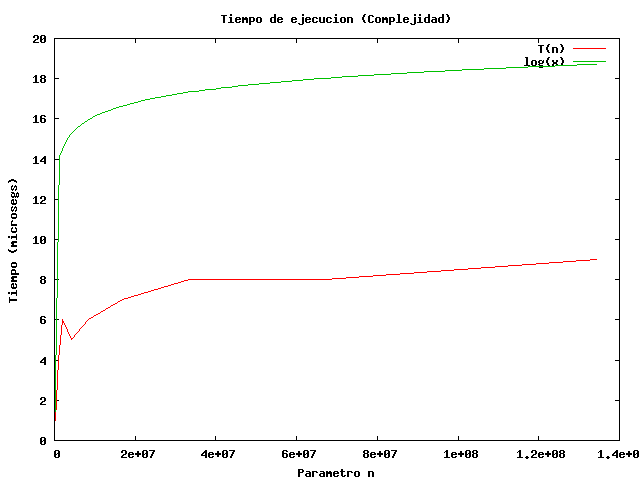
\includegraphics[width=0.7\textwidth]{Plots/Ej3-Complejidad.png}
% \begin{center}
% Figura 3.1
% \end{center}
% \end{center}

Como se puede observar en el gr\'afico, los tiempos de ejecuci\'on del algoritmo son muy bajos en relaci\'on al tama\~{n}o de la entrada. Esta fue la raz\'on por la que se descart\'o probar s\'olo casos peque\~{n}os para verificar la eficiencia del algoritmo y se opt\'o por analizar casos en el que el tama\~{n}o de la entrada creciera exponencialmente. A simple vista se puede observar que el gr\'afico de la funci\'on que mide el tiempo tiene el mismo comportamiento que la funci\'on de complejidad te\'orica. De este modo, adem\'as de la demostraci\'on te\'orica de la complejidad, se obtiene una prueba emp\'irica de que esta misma es correcta.

\section*{Conclusiones}

Este ejercicio nos hizo utilizar la t\'cnica de Divide and Conquer y nos mostr\'o varias de sus caracter\'isticas. La necesidad de utilizar 
esta t\'ecnica result\'o de la b\'usqueda de disminuir la complejidad lineal propuesta por la soluci\'on trivial.
	La complejidad obtenida muestra la relaci\'on que hay en ciertos algoritmos Divide and Conquer, entre el costo temporal de resolverlo 
y la cantidad de elementos de entrada. En este caso ni siquiera fue necesario leer cada uno de los elementos gracias a que cont\'abamos con
el orden de los vectores.
	En nuestro algoritmo el costo de cada una de las divisiones y cada una de las conquistas es contante, permitiendo que s\'olo 
la cantidad de llamadas a problemas m\'as peque\~{n}os defina la complejidad. Esta propiedad no logra s\'olo ser eficiente, sino que adem\'as, 
permite un c\'alculo sencillo de la complejidad temporal. En las pruebas emp\'iricas realizadas, puede observarse como el tiempo que toma realizar nuestro algoritmo,
es notablemente inferior al del tama\~{n}o de la entrada. Cabe destacar que nuestro algoritmo hace una cantidad similar de operaciones en todos los casos (para un mismo
tama\~{n}o de la entrada), ya que para calcular la mediana siempre debe llegar al caso base. Esto ayuda a la demostraci\'on de la correctitud del algortimo y lo hace 
m\'as natural. Puede observarse en el gr\'afico de nuestras pruebas, la ausencia de grandes picos, que muestra emp\'iricamente que para entradas de similar tama\~{n}o, el 
tiempo demandado ser\'a similar .
	Realizar este ejercicio tambi\'en nos mostr\'o la sencillez y la naturalidad con la que se pueden implementar los algoritmos divide and conquer mediante un 
m\'etodo recursivo, aunque claro, esto puede cambiar dependiendo de lo complejo que sea implementar la divisi\'on y la conquista. 
	En definitiva, se puede concluir que en ciertos casos,y en este en particular, los algoritmos Divide and Conquer son f\'aciles de implementar, eficientes en el peor caso, y es 
sencillo calcular su complejidad.


\end{document}